% Implementation 
\chapter{Implementation}
\label{sec:implement}

This section provides a brief overview of the experimental setup and aims to motivate the choice of datasets, libraries and frameworks.

\section{Scope and Limitations}
\label{sec:implement:scope}
Our research is concerned with graph-level prediction tasks on two types of \ac{gnn}, \ac{gcn} and \ac{gin}.
We implemented both networks as described in \cite{} and \cite{} respectively.
The implementation of \ac{gdc}





\section{Experimental Setup}
\label{sec:implement:setup}
\subsubsection{\Ac{gdc}}
Before we describe our implementation in Python, we look at the two proposed variants of \ac{gdc} and provide an intuition for them.
As stated previously, this version of \ac{gdc} allows drawing different random masks for each channel and edge independently, giving more flexibility and increasing the time and space complexity.
\begin{align*}
    H^{(l+1)}[:,j] & = \sigma \left(\sum_{i=1}^{f_{l}}\mathfrak{R}\left(A \odot Z_{i,j}^{(l)}\right)H^{(l)}[:,i]W^{(l)}[i,j]\right) \\
    \text{for } j  & = 1,..., f_{l+1}
\end{align*}
% Description and Intuition for GDC-eq4
Here, we calculate the new feature matrix $H^{(l+1)}$ by stacking the column vectors of each iteration. One can think of the calculations that are being performed as a $4$-dimensional matrix with the dimensions $n\times n\times f_{l}\times f_{l+1}$

To understand what is being done, we can look at what is being performed when calculating one column of the resulting matrix. First, a random mask is applied to the connection from the $i$-th to the $j$-th. Regarding node features communicating with each other, we look at the edge between the $i$-th and $j$-th features between connected nodes. By applying the random mask, we drop those connections selectively. Because we sample the random binary mask $Z$ $f_{l+1}$ times, one time for every feature in the $l+1$-th iteration, we differentiate between the connection $i \rightarrow j$ between two nodes and the connection $j \rightarrow i$ between the same two nodes. Thus, the same edge can be dropped as a connection and remain as a connection in the opposite direction. The masked adjacency is then multiplied by the corresponding column and weight.
One may think of it as performing a random sampling across each channel since in each iteration from $i=1$ to $f_{l+1}$, we perform multiplication with the $i-th$ column of $H$.

\begin{figure}[ht]
    \centering
    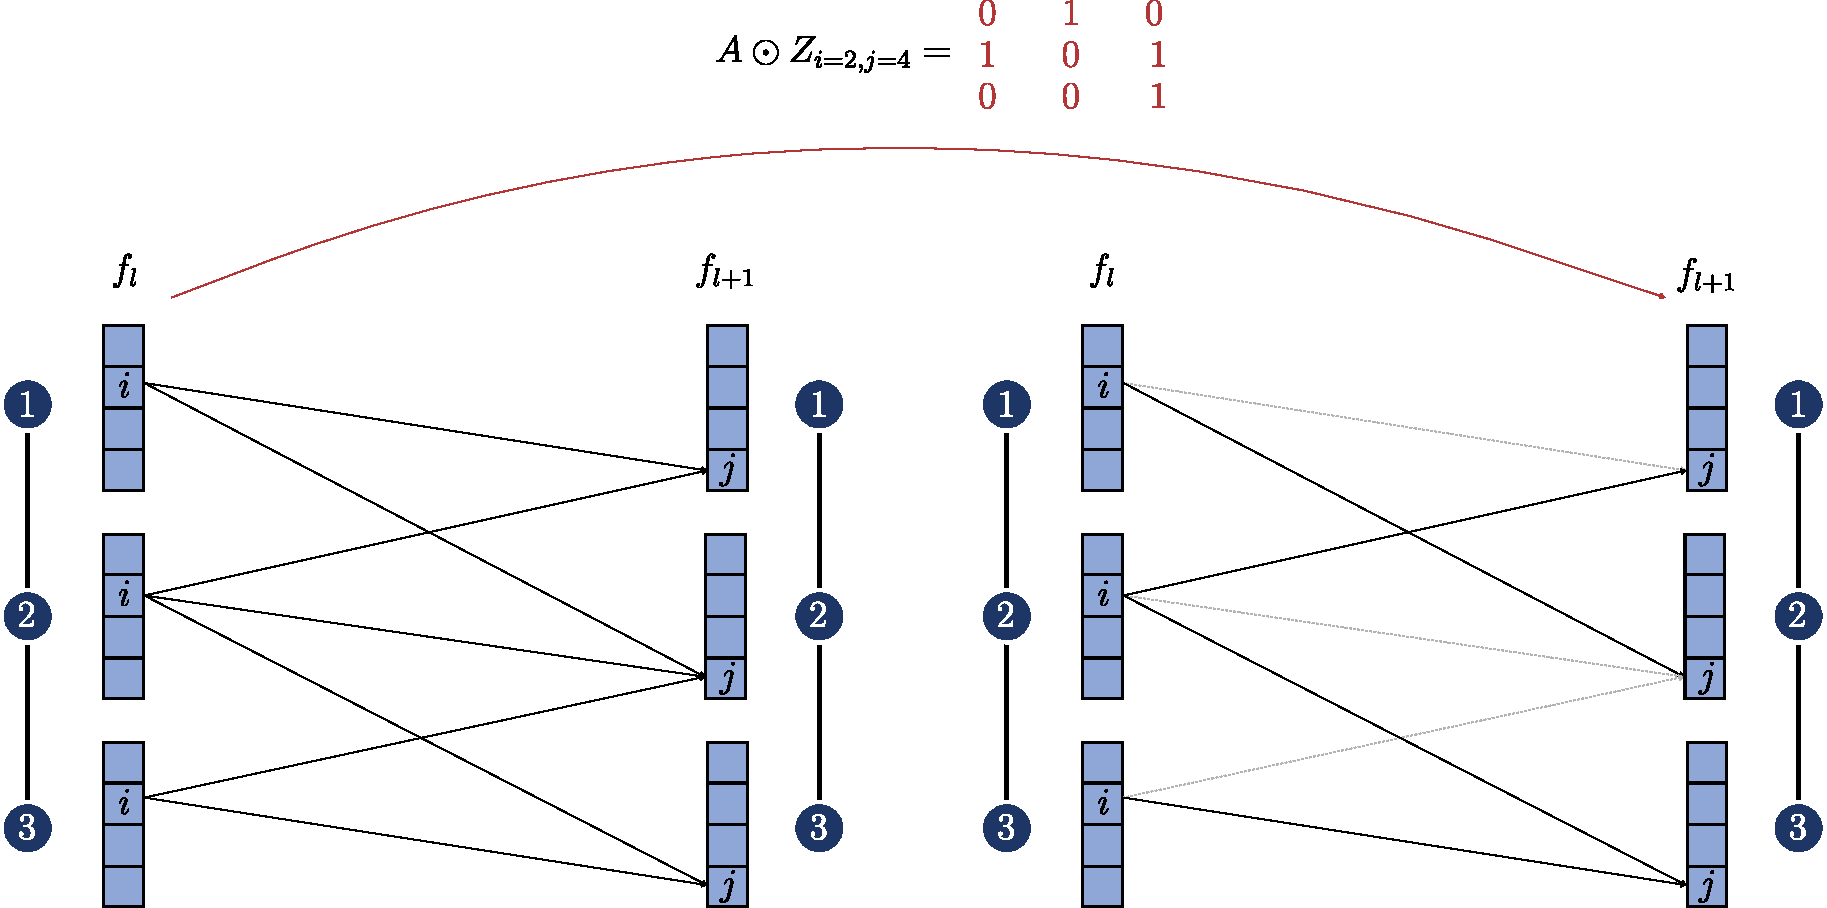
\includegraphics[width= 0.90\linewidth]{gfx/implementation/GDC-eq4.pdf}
    \caption{\Ac{gdc}Note: self connection are assumed}\label{fig:implementaion:GDC-eq4}
\end{figure}


As for the implementation of \ac{gdc}, we decided to implement the less complex version, as shown below, since this implementation reduces the runtime completely and is also the one that was originally implemented for testing the efficacy of \ac{gdc}
\begin{align}
    H^{(l+1)} = \sigma(\sum_{i= 1}^{f_{l}}\mathfrak{N}(A \odot Z_{i}^{(l)})H^{(l)}[:,i] W^{(l)}[i,:])
\end{align}

Here, we compute the new feature matrix in one go, instead of doing $f_{l}$ iterations for all $f_{l}$ columns.
\begin{figure}[ht]
    \centering
    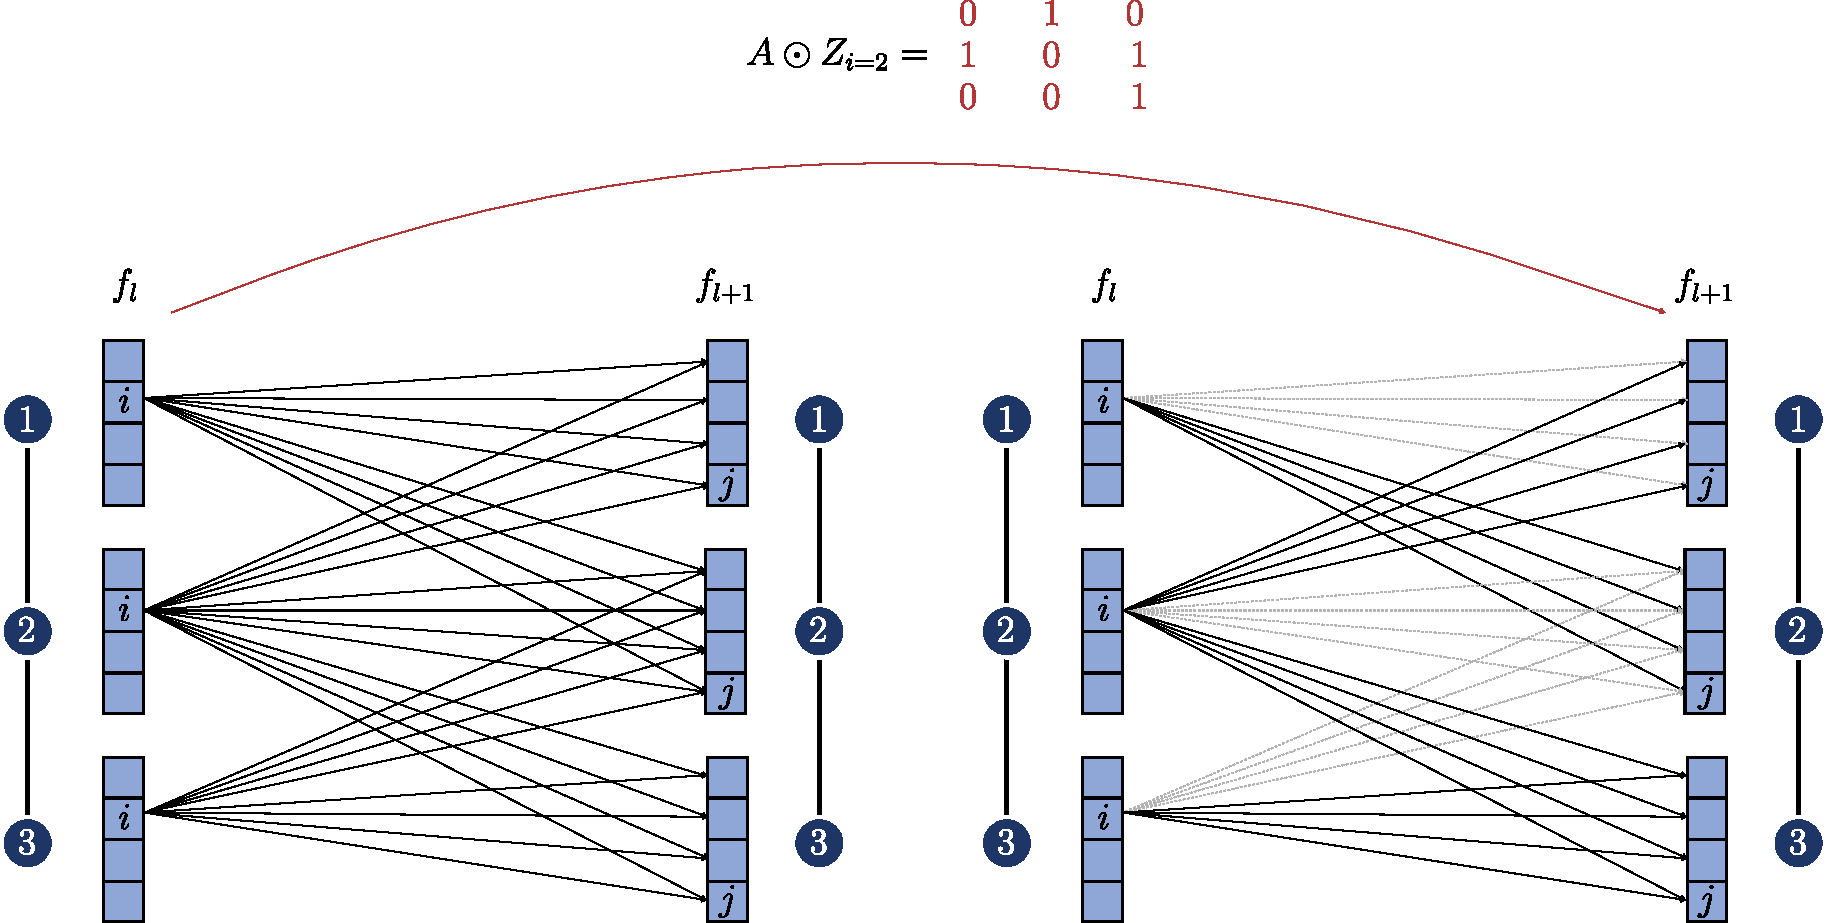
\includegraphics[width= 0.90\linewidth]{gfx/implementation/GDC-eq5.pdf}
    \caption{Originally proposed \ac{gdc}Note: self connection are assumed}\label{fig:implementaion:GDC-eq5}
\end{figure}

\subsection{Choice of Frameworks}
\label{sec:implement:setup:choice}
Below we give a quick overview of used daasets and frameworks and motivate the choice.


\subsubsection{Datasets}
\label{sec:implement:setup:choice:data}
% Datasets - OGB 
Despite the fact, that machine learning on graph-structured data is carried out in many areas and has many interesting use cases ranging from social networks, to molecular graphs, to manifolds, to source code~\cite{Hu2020},
there does not exist and unified framework for working with graph-structured data. Furthermore commonly-used datasets and evaluation procedures suffer from multiple issues, that negatively affect the quality of predictions and the reliability of evaluations of models.
Machine learning algorithms rely heavily on data. In order for a \ac{gnn} to be able to make accurate predictions, there is need for a sufficient amount of properly prepared training data. To be able to compare different models against each other there is need of standardized splitting and evaluation methods.

% Problems overview 
Today, most of the frequently-used
graph datasets are extremely small compared to graphs found in
real applications. Same datasets, such as Cora, CiteSeer and PubMed are used again and again to train various models leading to poor scalability in the majority of cases. Small datasets also make it hard to rigorously evaluate data-hungry models, such as \acfp{gnn}. The performance of a \ac{gnn} on these datasets is often unstable and nearly statistically identical to each other, due to the small number of samples the models are trained and evaluated on~\cite{Kipf2017,Xu2019, Hu2020}.

% OGB benefits  
\textbf{\Ac{ogb}} offers a wide range of different-sized graph-datasets from different domains for a variety of different classification tasks and provides an unified pipeline for working with the datasets in \ac{ml} tasks.
The unified experimental protocol with standardized dataset splits, evaluation metrics and cross-validation protocols makes it easy to compare perfromance reported across various studies~\cite{Hu2020}.

% overview of standardized pipeline 
% graphic ? 
Working with \ac{ogb} consists of following steps:

\begin{enumerate}
    \item \Ac{ogb} provides realistic, different-scaled graph benchmark datasets that cover different prediction tasks, are from diverse application.
    \item Dataset processing and splitting is fully automated. \Ac{ogb} data loaders automatically download and process graphs and further split the datasets in a standardized manner. This is compatible with multiple libraries and a library-agnostic option is also provided.
    \item This step includes developing an \ac{ml} model to train on the ogb datasets.
    \item  \Ac{ogb} evaluates the model in a dataset-dependent manner, and outputs the model performance appropriate for the task at hand.
    \item \Ac{ogb} provides public leaderboards to keep track of recent advances.
\end{enumerate}

\begin{figure}[H]
    \centering
    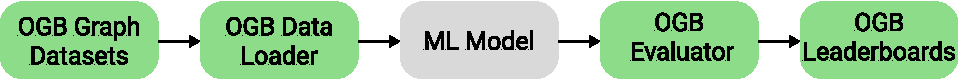
\includegraphics[width= 0.90\linewidth]{gfx/implementation/OGB_pipeline}
    \caption{\textbf{Overview of the standardized OGB pipeline} adapted from \cite{Hu2020}}\label{fig:implement:pipeline}
\end{figure}


% Introduction of MAD 
\subsubsection{Metrics}
\label{sec:implement:setup:choice:metrics}
To be able to make systematic and quantative statements about the positive effects on oversmoothing by using different regularization techniques, one has to be able to monitor the smoothness of nodes at different execution steps during training. Therefore, a choice of a suitable metric is of great importance, as it helps to access the extent of the effect produced by various regularization techniques and compare them against each other in terms of efficacy.
% TODO: CITE

\textbf{\Ac{mad}} ~\cite{Chen2020} is a metric for smoothness, the similarity of graph nodes representations. In that sence over-smoothness is the similarity of nodes representations among different classes.
While smoothing to some extent is desired(we assume spatial similarity between nodes), mixing features of nodes with different lables over several iterations leads to oversmoothing.

It is therefore important to differentiate between different types of messages between nodes. Signal/information is the messaging of nodes, which share the same class/label, i.e., intra-class communication and noize denotes intra-class comunication. Having too many inter-class edges leads to much noise by encorporating messages from other classes, which results in oversmoothing.

Because of that it is crucial to have a measure of the quality of the recieved messages. A way to do that is to consider the information-to noise ratio i.e., the fraction of intra-class node pairs and all node pairs that have interaction trough \ac{gnn} model. That way it is possible to differentiate between remote and neihbouring nodes and calculate the \textbf{\ac{madg}}, which is strongly positive correlated with a models accuracy.

% Formal definition 
\ac{mad} is calculated as follows:

Given the graph representation matrix $H \in \mathbb{R}^{n \times h}$ we
first obtain the distance matrix $D \in \mathbb{R}^{n \times n}$ for $H$ by
computing the cosine distance between each node pair.

\begin{align*}
    D_{i,j} = 1 - \frac{H_{i,:} \cdot H_{j,:}}{\mid H_{i,:}\mid  \cdot \mid H_{j,:}\mid} \; \;  i,j \in [1,2, \dots, n],
\end{align*}

where $H_{k}$ is the $k$-th row of $H$. The reason to use cosine distance is that cosine distance is not affected by the absolute value of the node vector,
thus better reflecting the smoothness of graph representation. Then we filter the target node pairs by element-wise multiplication $D$ with a mask matrix $M^{tgt}$

\begin{align*}
    D^{tgt} = D \odot M^{tgt},
\end{align*}
where $\odot$ denotes the element-wise mutliplication: $M^{tgt} \in \{0,1\}^{n \times n}; M_{i,j}^{tgt}= 1$ only if node pair $(i,j)$ is the target one.
Next we access the average distance $\bar{D}^{tgt}$ for non-zero values along each row in $D^{tgt}:$

\begin{align*}
    \bar{D}_{t}^{tgt} = \frac{\sum_{j=0}^{n}D_{i,j}^{tgt}}{\sum_{j=0}^{n}\mathds{1}(D_{i,j}^{tgt})}
\end{align*}
where where 1(x) = 1 if x > 0 otherwise 0. Finally, the MAD
value given the target node pairs is calculated by averaging
the non-zero values in
tgt
% Intuition behind all this 
\Ac{mad} gives access to the smoothness of a node and pairs of nodes throughout iterations, which makes it easy to "track down" over smoothing.
First, the cosine similarity is calculated, showing how similar the corresponding feature vectors are. By subtracting the cosine similarity from one, we get the cosine distance, which tells us the difference between the nodes.


% graphic signal/ information & noise 
\subsection{Implementation of Regularization Techniques}
\label{sec:implement:setup: regularization}

% Descrepancy between Paper and our implementation 



% Implementation of Regularization 
The four regularization techniques, as described in \ref{sec:related:pred:regularization}, can be described using two parameters illustrated in the table below: Is the regularization happening row-wise, and do we gather the values before applying the regularization?
\begin{center}
    \begin{tabular}{lll}
        \toprule
        \textbf{Regularization} & \textbf{row-wise?} & \textbf{gather first?} \\
        \midrule
        \acf{do}                & false              & false                  \\
        \acf{de}                & true               & true                   \\
        \acf{ns}                & true               & false                  \\
        \acf{gdc}               & false              & true                   \\

        \bottomrule
    \end{tabular}
\end{center}
\subsubsection{gather, scatter, sparcity}
In our implementation, we make use of TensorFlow gather and scatter operations:
The gather operation in TensorFlow extracts specific elements from a tensor along a given axis. Given an input tensor and a list of indices, the gather operation selects elements based on the provided indices from the input tensor. Given a tensor representing node features in a graph and a list of node indices, the gather operation extracts the corresponding node features. The gather operation can extract node features, adjacency information, or other relevant data based on specific graph node indices.

The scatter operation in TensorFlow is the inverse of the gather operation. It updates the elements of an existing tensor based on the provided indices. Given an input tensor, a list of indices, and a tensor containing values, the scatter operation replaces elements in the input tensor at the specified indices with the corresponding values from the values tensor.
Gather and scatter operations are crucial for tasks involving graph neural networks \acp{gnn} where information aggregation and dissemination across nodes are essential. Information from nodes or subgraphs is gathered and aggregated for graph classification tasks to represent the entire graph.\acp{gnn} can use gather operations to pool information from nodes and perform graph-level predictions.

\subsection{Finding the Best Set of hyperparameters}
\label{sec:implement:setup: gridsearch}

For hyperparameter optimization, we use grid search \ac{gs}~\cite{Lorenzo2017,Yang2020,Zoeller2021}.\Ac{gs} is a model-free method of automated hyperparameter selection, which systematically explores the configuration space performing an exhaustive search.
\begin{enumerate}
    \item Poor scalability for large configuration spaces due to its exponential complexity in the number of hyperparameters and corresponding values. Assuming that there are k parameters, and each of them has n distinct values, its computational complexity is $O(n^{k})$
    \item Lack of consideration of the hierarchical hyperparameter structure leads to many redundant configurations.
\end{enumerate}
Despite its two major drawbacks,\ac{gs} is well-suitable for small search spaces and can easily be implemented and parallelized.